\documentclass{article}

% if you need to pass options to natbib, use, e.g.:
%     \PassOptionsToPackage{numbers, compress}{natbib}
% before loading neurips_2018

% ready for submission
% \usepackage{neurips_2018}

% to compile a preprint version, e.g., for submission to arXiv, add add the
% [preprint] option:
%     \usepackage[preprint]{neurips_2018}

% to compile a camera-ready version, add the [final] option, e.g.:
     \usepackage[final]{neurips_2018}

% to avoid loading the natbib package, add option nonatbib:
%     \usepackage[nonatbib]{neurips_2018}

\usepackage[utf8]{inputenc} % allow utf-8 input
\usepackage[T1]{fontenc}    % use 8-bit T1 fonts
\usepackage{hyperref}       % hyperlinks
\usepackage{url}            % simple URL typesetting
\usepackage{booktabs}       % professional-quality tables
\usepackage{amsfonts}       % blackboard math symbols
\usepackage{nicefrac}       % compact symbols for 1/2, etc.
\usepackage{microtype}      % microtypography
\usepackage{amsmath}
\usepackage{amssymb}
\usepackage{graphicx}
\usepackage{subcaption}
\usepackage{booktabs}
\newcommand{\pd}[2]{\frac{\partial #1}{\partial #2}}

\title{Deep Learning\\Assignment 1: MLPs, CNNs and Backpropagation}

% The \author macro works with any number of authors. There are two commands
% used to separate the names and addresses of multiple authors: \And and \AND.
%
% Using \And between authors leaves it to LaTeX to determine where to break the
% lines. Using \AND forces a line break at that point. So, if LaTeX puts 3 of 4
% authors names on the first line, and the last on the second line, try using
% \AND instead of \And before the third author name.

\author{%
  Daniel Daza\\
  University of Amsterdam\\
  \texttt{daniel.dazacruz@student.uva.nl} \\
  % examples of more authors
  % \And
  % Coauthor \\
  % Affiliation \\
  % Address \\
  % \texttt{email} \\
  % \AND
  % Coauthor \\
  % Affiliation \\
  % Address \\
  % \texttt{email} \\
  % \And
  % Coauthor \\
  % Affiliation \\
  % Address \\
  % \texttt{email} \\
  % \And
  % Coauthor \\
  % Affiliation \\
  % Address \\
  % \texttt{email} \\
}

\begin{document}
% \nipsfinalcopy is no longer used

\maketitle

\begin{abstract}
Neural networks are flexible function approximators that have a wide range of applications in artificial intelligence. In this work we derive the gradient equations that are needed to train a Multi-Layer Perceptron (MLP), and we implement and test its performance on the task of image classification. We additionally derive the gradient equations for the Batch-Normalization layer. Lastly, we implement a Convolutional Neural Network (CNN) and test it on the same task. We find that the MLP can generalize to samples outside the training set by using regularization techniques, albeit at a lower accuracy; and that networks with more parameters and appropriate prior structure, such as CNNs, yield better performance.
\end{abstract}

\section{MLP, backpropagation and NumPy implementation}

\subsection{Analytical derivation of gradients}

\subsection*{Question 1.1 a)}

\subsubsection*{Cross-entropy loss}

Since the loss only depends on $x_i$ if $t_i = 1$, this gradient is a vector of zeros except in the position given by $\arg\max(t)$:

\begin{align}
\left(\frac{\partial L}{\partial x^{(N)}} \right)_i &=
\left\lbrace
\begin{matrix}
0 &\text{ if } i \neq \arg\max(t)\\
\frac{\partial}{\partial x_i^{(N)}}\left(-\log x_i^{(N)}\right) &\text{ if } i = \arg\max(t)\\
\end{matrix}
\right.\\
&= \left\lbrace
\begin{matrix}
0 &\text{ if } i \neq \arg\max(t)\\
-\frac{1}{x_i^{(N)}} &\text{ if } i = \arg\max(t)\\
\end{matrix}
\right.
\end{align}


Therefore, the gradient vector can be obtained by element-wise multiplication with the targets vector:
\begin{equation}
\frac{\partial L}{\partial x^{(N)}} = -t\odot\frac{1}{x^{(N)}}
\end{equation}


\subsubsection*{Softmax layer}


\begin{align}
\left(\frac{\partial x^{(N)}}{\tilde{x}^{(N)}}\right)_{ij}
&= \frac{\partial x^{(N)}_i}{\tilde{x}^{(N)}_j}\\
&=
\frac{\partial}{\partial\tilde{x^{(N)}_j}}\left(
\frac{\exp(\tilde{x}^{(N)})_i}{\sum_{k=1}^{d_N} \exp(\tilde{x}^{(N)})_k}
\right)\\
&=
\frac{\partial}{\partial\tilde{x^{(N)}_j}}\left(
\frac{\exp(\tilde{x}^{(N)})_i}{Z}
\right)\\
&=
\frac{Z\frac{\partial}{\partial\tilde{x}_j}\exp(\tilde{x}^{(N)})_i-\exp(\tilde{x}^{(N)})_i\frac{\partial}{\partial\tilde{x}_j}Z}{Z^2}\\
&=
\frac{Z\frac{\partial}{\partial\tilde{x}_j}\exp(\tilde{x}^{(N)})_i-\exp(\tilde{x}^{(N)})_i\frac{\partial}{\partial\tilde{x}_j}\sum_{k=1}^{d_N} \exp(\tilde{x}^{(N)}_k)}{Z^2}\\
&=
\frac{Z\frac{\partial}{\partial\tilde{x}_j}\exp(\tilde{x}^{(N)})_i-\exp(\tilde{x}^{(N)})_i \exp(\tilde{x}^{(N)}_j)}{Z^2}\\
&=
\frac{\frac{\partial}{\partial\tilde{x}_j}\exp(\tilde{x}^{(N)})_i}{Z}-\frac{\exp(\tilde{x}^{(N)})_i \exp(\tilde{x}^{(N)}_j)}{Z^2}\\
&=
\frac{\frac{\partial}{\partial\tilde{x}_j}\exp(\tilde{x}^{(N)})_i}{Z}-\frac{\exp(\tilde{x}^{(N)})_i}{Z}\frac{\exp(\tilde{x}^{(N)}_j)}{Z}\\
&=
\frac{\frac{\partial}{\partial\tilde{x}_j}\exp(\tilde{x}^{(N)})_i}{Z}-\text{softmax}(\tilde{x}^{(N)})_i\text{softmax}(\tilde{x}^{(N)})_j\\
&=
\left\lbrace
\begin{matrix}
-\text{softmax}(\tilde{x}^{(N)})_i\text{softmax}(\tilde{x}^{(N)})_j \text{ if } i\neq j\\
\frac{\exp(\tilde{x}^{(N)})_j}{Z}-\text{softmax}(\tilde{x}^{(N)})_i\text{softmax}(\tilde{x}^{(N)})_j\text{ if } i = j\\
\end{matrix}
\right. \\
&=
\left\lbrace
\begin{matrix}
-x^{(N)}_i x^{(N)}_j \text{ if } i\neq j\\
x^{(N)}_j-x^{(N)}_i x^{(N)}_j\text{ if } i = j\\
\end{matrix}
\right. \\
\end{align}


The Jacobian is then:

\begin{equation}
\frac{\partial x^{(N)}}{\partial\tilde{x}^{(N)}} =
\text{diag}(x^{(N)})-x^{(N)}{x^{(N)\top}}
\end{equation}

\subsubsection*{ReLU activation}

\begin{align}
\left(\frac{\partial x^{(l<N)}}{\partial\tilde{x}^{(l<N)}}\right)_{ij}
&=
\frac{\partial}{\partial\tilde{x}^{(l)}_j}\max(0,\tilde{x}^{(l)}_i)\\
&=
\left\lbrace
\begin{matrix}
1&\quad\text{if } i = j\text{ and } \tilde{x}^{(l)}<0\\
0&\quad\text{otherwise} \\
\end{matrix}
\right.
\end{align}

If we let $\mathbb{I}[s]$  be an indicator variable equal to 1 when the element-wise statement $s$ is true, the Jacobian can be written as follows:
\begin{equation}
\frac{\partial x^{(l<N)}}{\partial\tilde{x}^{(l<N)}} = \text{diag}(\mathbb{I}[\tilde{x}^{(l)}>0])
\end{equation}

\subsubsection*{Linear layer}


\begin{align}
\frac{\partial\tilde{x}^{(l)}}{\partial x^{(l-1)}}
&=
\frac{\partial}{\partial x^{(l-1)}}(W^{(l)}x^{(l-1)}+b^{(l)})\\
&= W^{(l)}
\end{align}



Let $W^{(l)}_{i:}$ be a slice containing the $i$-th row of $W^{(l)}$. Then we have:

\begin{align}
\left(\frac{\partial\tilde{x}^{(l)}}{\partial W^{(l)}}\right)_{ijk}
&= \frac{\partial\tilde{x}^{(l)}_i}{\partial W^{(l)}_{jk}}\\
&=
\frac{\partial}{\partial W^{(l)}_{jk}}(W^{(l)}x^{(l-1)}+b^{(l)})_i \\
&=
\frac{\partial}{\partial W^{(l)}_{jk}}({W^{(l)}_{i:}}^\top x^{(l-1)}+b^{(l)}_i) \\
&=
\left\lbrace
\begin{matrix}
x^{(l-1)}_k\quad &\text{if } i = j\\
0\quad &\text{otherwise}
\end{matrix}
\right.
\end{align}

Lastly,

\begin{align}
\left(\frac{\partial \tilde{x}^{(l)}}{\partial b^{(l)}}\right)_{ij}
&=
\frac{\partial}{\partial b^{(l)}_j}(W^{(l)}x^{(l-1)}+b^{(l)})_i \\
&=
\left\lbrace
\begin{matrix}
1\quad &\text{if } i = j\\
0\quad &\text{otherwise}
\end{matrix}
\right.
\end{align}

\subsection*{Question 1.1 b)}

\subsubsection*{Softmax backward}

\begin{align}
\frac{\partial L}{\partial\tilde{x}^{(N)}}
&=
\frac{\partial L}{\partial x^{(N)}}\frac{\partial x^{(N)}}{\partial \tilde{x}^{(N)}}\\
&=
\frac{\partial L}{\partial x^{(N)}}\left(\text{diag}(x^{(N)})-x^{(N)}{x^{(N)\top}}\right)
\end{align}

\subsubsection*{ReLU backward}

\begin{align}
\frac{\partial L}{\partial \tilde{x}^{(l<N)}} &= \frac{\partial L}{\partial x^{(l)}}\frac{\partial x^{(l)}}{\partial\tilde{x}^{(l)}}\\
&= \frac{\partial L}{\partial x^{(l)}}\text{diag}(\mathbb{I}[\tilde{x}^{(l)}>0])\\
&= \frac{\partial L}{\partial x^{(l)}}\odot\mathbb{I}[\tilde{x}^{(l)}>0]
\end{align}

\subsubsection*{Linear backward}

\begin{align*}
\frac{\partial L}{\partial x^{(l<N)}} &= \frac{\partial L}{\partial\tilde{x}^{(l+1)}}\frac{\partial\tilde{x}^{(l+1)}}{\partial x^{(l)}} \\
&= \frac{\partial L}{\partial\tilde{x}^{(l+1)}}W^{(l+1)}
\end{align*}

From the chain rule we have:
\begin{align}
\left(\frac{\partial L}{\partial W^{(l)}}\right)_{ij} &= \sum_k\frac{\partial L}{\partial \tilde{x}^{(l)}_k}\frac{\partial \tilde{x}^{(l)}_k}{\partial W_{ij}}\\
&= \frac{\partial L}{\partial \tilde{x}^{(l)}_i}x^{(l-1)}_j
\end{align}

Therefore, the gradient with respect to $W^{(l)}$ can be written as an outer product:
\begin{align}
\frac{\partial L}{\partial W^{(l)}} &= \frac{\partial L}{\partial\tilde{x}^{(l)}}x^{(l-1)\top}
\end{align}

\begin{align}
\left(\frac{\partial L}{\partial b^{(l)}}\right)_i &= \sum_j \frac{\partial L}{\partial\tilde{x}^{(l)}_j} \frac{\partial\tilde{x}^{(l)}_j}{\partial b^{(l)}_i}\\
&=
\frac{\partial L}{\partial\tilde{x}^{(l)}_i}
\end{align}

Therefore:
\begin{equation}
\frac{\partial L}{\partial b^{(l)}} = \frac{\partial L}{\partial\tilde{x}^{(l)}}
\end{equation}

\subsection*{Question 1.1 c)}

Let us assume that when using batches, the $B$ samples and targets are arranged in the rows of matrices $X^{(0)}$ and $T$, and for any linear module the output is calculated as $X^{(l-1)}W^{(l)\top} + b^{(l)}$. In this case, the output of the module will be a matrix as well.

When using a single sample, we obtained the following gradient for the cross-entropy loss:

\begin{equation*}
\frac{\partial L}{\partial x^{(N)}} = -t\odot\frac{1}{x^{(N)}}
\end{equation*}

This vector is used during backpropagation to calculate the next gradients. In the new batched formulation, it turns into is a matrix that we can arrange so that the number of rows equals the number of samples in the batch:

\begin{equation}
-T\odot \frac{1}{X^{(N)}} = 
\begin{bmatrix}
-T_{1:}\odot\frac{1}{X^{(N)}_{1:}}\\
-T_{2:}\odot\frac{1}{X^{(N)}_{2:}}\\
\vdots\\
-T_{B:}\odot\frac{1}{X^{(N)}_{B:}}
\end{bmatrix}
\end{equation}

By matrix multiplication, every backward step of a module will then produce a matrix with one row per sample. When calculating the gradients of the parameters, each sample in the batch will produce a gradient matrix for $W^{(l)}$ and a gradient vector for $b^{(l)}$ via brodcasting of matrix multiplication. These gradient arrays can be averaged across the batch axis before updating the parameters.

\subsection*{Question 1.2: NumPy implementation}
\label{sec:numpy}

The previous equations were used to implement an MLP with the NumPy library to solve an image classification problem with the CIFAR-10 dataset \cite{krizhevsky2009learning}, with a training set of 50,000 images and 10,000 images for testing. We trained a 2-layer MLP with 100 units in the hidden layer and the ReLU activation function, a batch size of 200, Stochastic Gradient Descent (SGD) with a learning rate of 1$\times$10$^{-3}$, for 1,500 steps. To evaluate the performance of the classifier we use the accuracy score.

We obtained an accuracy of 46.6\% in the test set. During training, we observed that the test set obtained a value of 48.8\% after 1,000 iterations, and later decreased, which indicates a sign of overfitting. This can also be seen in the loss and accuracy curves, shown in Figure \ref{fig:mlp_curves}, where a gap between the training and test curves starts to appear towards the end of training. We can also see that at 1,500 iterations the curves appear to stagnate, suggesting that training for more iterations would further decrease the performance on the test set due to overfitting.

\begin{figure}[t]
\begin{subfigure}{0.49\textwidth}
\centering
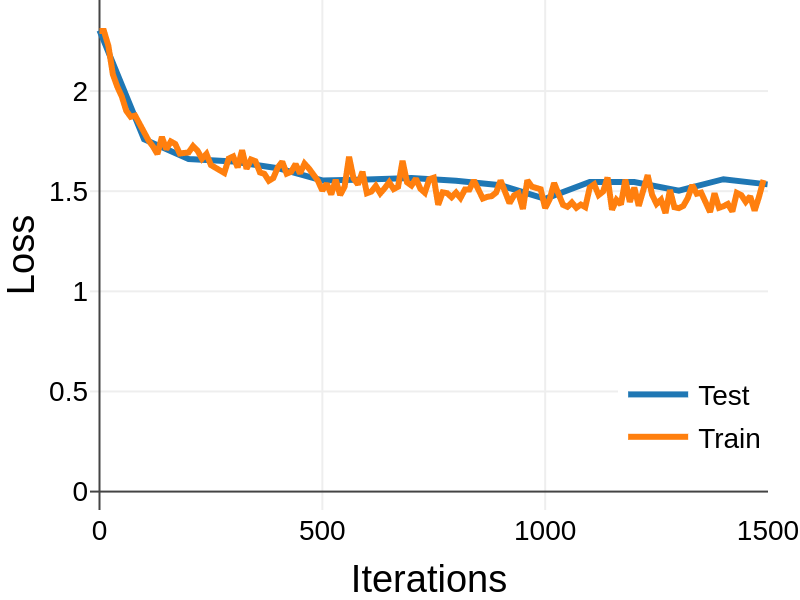
\includegraphics[scale=0.22]{img/mlp-loss}
\caption{}
\end{subfigure}
\begin{subfigure}{0.49\textwidth}
\centering
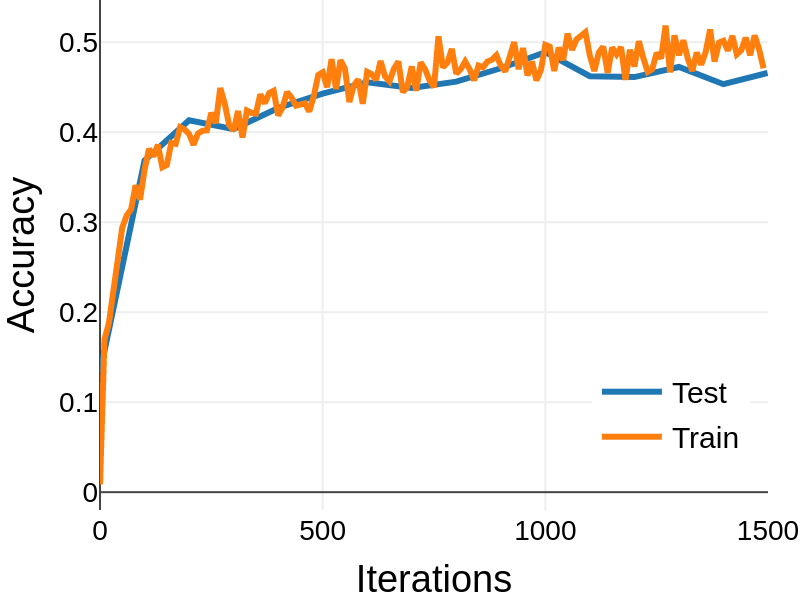
\includegraphics[scale=0.22]{img/mlp-acc}
\caption{}
\end{subfigure}
 \caption{Curves for (a) the loss, and (b) accuracy on the training and test splits, when training an MLP for image classification with NumPy. Training values are averaged over 10 steps, and test values are measured every 100 steps.}
\label{fig:mlp_curves}
\end{figure}

\section{PyTorch MLP}

\subsection*{Question 2}
We implemented the same MLP using the PyTorch library, and obtained an accuracy of 43.7\% with the same hyperparameters as the NumPy implementation. We attribute the difference to the initialization strategy, as in the NumPy implementation we initialize the weights from a Gaussian distribution with a mean of 0 and a standard deviation of 0.0001, whereas by default PyTorch uses the \textit{He initialization} strategy \cite{he2015delving}.

In order to improve the performance of the model, we experiment with modifications to the architecture and training procedure. Increasing the number of parameters allows the model to represent more complex functions \cite{hornik1991approximation}, and arranging these into different layers imposes a hierarchical inductive bias that has shown to improve the generalization properties of neural networks \cite{bengio2007greedy,bengio2013representation}. However, the increased complexity of the model also increases its propensity to overfitting to the training data, and methods like regularizing the $\ell_2$-norm of the weights, and dropout \cite{srivastava2014dropout} have been proposed to overcome this outcome.

Another important component in training neural networks is the optimization algorithm used to minimize the loss. While our first experiments use SGD, other alternatives have been proposed that improve the convergence speed, such as the use of momentum  \cite{polyak1964momentum,sutskever2013nesterov} and second order moment estimation, as used in the Adam algorithm \citep{krizhevsky2009learning}.

Based on the previous reasons, we experiment with a model with three layers. We vary the number of units in the first layer, and we fix the second layer with 400 units. We add dropout to the output of the second layer, and we train the neural network with Adam, including weight decay regularization. We train for 4,000 iterations, which we observed was necessary to achieve a stable convergence of the training loss. To find the best set of hyperparameters, we run grid search according to the values listed in Table \ref{tab:hparams}.

\begin{table}[t]
\centering
\caption{Hyperparameter settings for the grid search carried out for the PyTorch implementation of the MLP. The best values are shown for the model with the highest accuracy on the test set.}
\label{tab:hparams}
\begin{tabular}{lll}
\bf Hyperparameter & \bf Values  & \bf Best\\
\specialrule{.1em}{.05em}{.05em}
Units in the first layer & $\lbrace 400, 600, 1000\rbrace $ & $600$ \\
Weight decay & $\lbrace 0.1, 0.01, 0.001\rbrace$ & $0.1$ \\
Dropout & $\lbrace 0.1, 0.2, 0.5\rbrace$ & $0.1$ \\
Learning rate & $\lbrace 1\times 10^{-3}, 5\times 10^{-4}, 1\times 10^{-4}\rbrace$ & $1\times 10^{-4}$
\end{tabular}
\end{table}

Table \ref{tab:hparams} also includes the best set of hyperparameters, which yielded an accuracy of 54.2\% in the test set. We note that the best model is not the one with more parameters, but a model in the mid range that is also regularized both with weight decay and dropout. The loss and accuracy curves for this model are shown in Figure \ref{fig:torch_curves}. We can see that the regularization methods effectively prevent the model from overfitting, as the gap between the training and test curves is controlled as the number of iteration increases. The accuracy curves also suggest that training for more iterations could further improve the performance on the test set.

\begin{figure}[t]
\begin{subfigure}{0.49\textwidth}
\centering
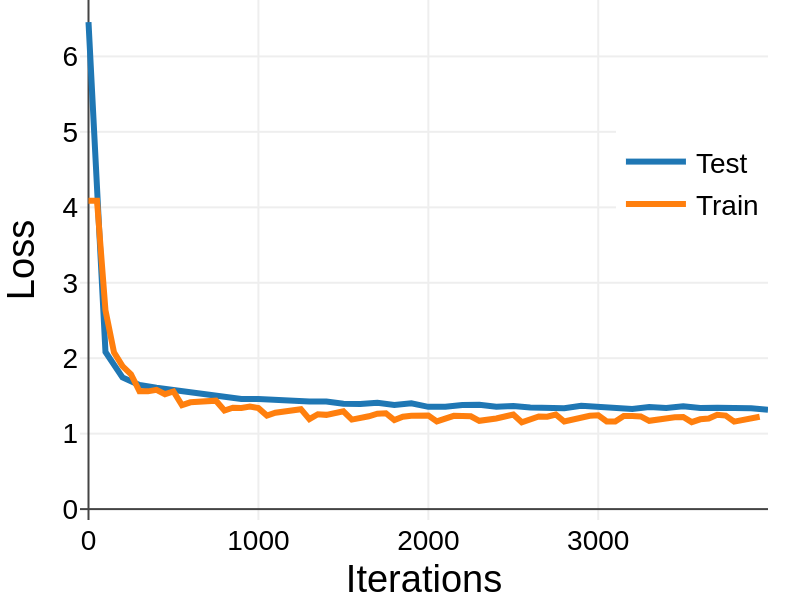
\includegraphics[scale=0.22]{img/torchmlp-loss}
\caption{}
\end{subfigure}
\begin{subfigure}{0.49\textwidth}
\centering
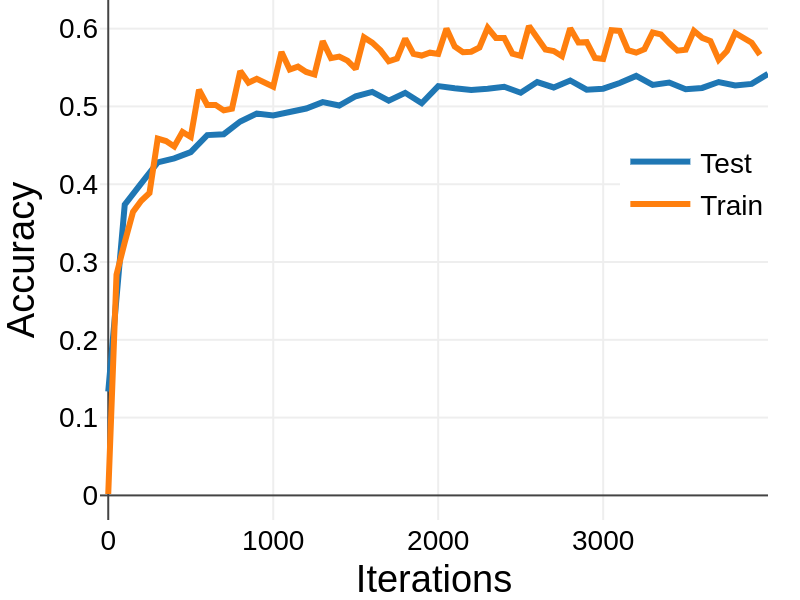
\includegraphics[scale=0.22]{img/torchmlp-acc}
\caption{}
\end{subfigure}
 \caption{Curves for (a) the loss, and (b) accuracy on the training and test splits, when training an MLP for image classification with PyTorch. Training values are averaged over 10 steps, and test values are measured every 100 steps.}
\label{fig:torch_curves}
\end{figure}

\section{Batch Normalization}

We reproduce the forward propagation equations for the batch normalization layer here for future reference:

\begin{align}
\mu_i &= \frac{1}{B}\sum_{s=1}^B x_i^s \\
\sigma_i &= \frac{1}{B}\sum_{s=1}^B (x_i^s - \mu_i)^2 \\
\hat{x}_i^s &= \frac{x_i^s -  \mu_i}{\sqrt{\sigma_i^2 + \epsilon}} \\
y_i^s &= \gamma_i\hat{x}_i^s + \beta_i
\end{align}

\subsection*{Question 3.1}

For this question, the forward propagation equations were implemented in PyTorch.

\subsection*{Question 3.2 a)}

We now derive the backpropagation equations for the batch normalization layer. We are interested in the gradients of the loss with respect to $\gamma$, $\beta$, and $x$. We assume that the gradient with respect to the module output, $y$, is already provided by the layer following it.

\begin{align*}
\left(\pd{L}{\gamma}\right)_j &= \pd{L}{\gamma_j} \\
&=
\sum_s\sum_i\pd{L}{y_i^s}\pd{y_i^s}{\gamma_j} \\
&=
\sum_s\pd{L}{y_j^s}\pd{y_j^s}{\gamma_j} \\
&= \sum_s\pd{L}{y_j^s}\pd{}{\gamma_j}(\gamma_j\hat{x}_j^s+\beta_j) \\
&= \sum_s\pd{L}{y_j^s}\hat{x}_j^s
\end{align*}

\begin{align*}
\left(\pd{L}{\beta}\right)_j &= \pd{L}{\beta_j} \\
&=
\sum_s\sum_i\pd{L}{y_i^s}\pd{y_i^s}{\beta_j} \\
&=
\sum_s\pd{L}{y_j^s}\pd{y_j^s}{\beta_j} \\
&= \sum_s\pd{L}{y_j^s}\pd{}{\beta_j}(\gamma_j\hat{x}_j^s+\beta_j) \\
&= \sum_s\pd{L}{y_j^s}
\end{align*}

\begin{align}
\left(\pd{L}{x}\right)_{jk} &= \pd{L}{x_j^k} \notag \\
&= \pd{L}{y_j^k}\pd{y_j^k}{\hat{x}_j^k}\pd{\hat{x}_j^k}{x_j^k} + \sum_s \pd{L}{y_j^s}\pd{y_j^s}{\hat{x}_j^s}\left(\pd{\hat{x}_j^s}{\mu_j}\pd{\mu_j}{x_j^k} + \pd{\hat{x}_j^s}{\sigma_j^2}\left[\pd{\sigma_j^2}{x_j^k} + \pd{\sigma_j^2}{\mu_j}\pd{\mu_j}{x_j^k} \right] \right) \label{eq:dldx}
\end{align}

The derivatives required in the last equation are derived next:

\begin{align*}
\pd{y_j^k}{\hat{x}_j^k} &= \pd{}{\hat{x}_j^k}(\gamma_j\hat{x}_j^k + \beta_j) \\
&= \gamma_j
\end{align*}

\begin{align*}
\pd{\hat{x}_j^k}{x_j^k} &= \pd{}{x_j^k}\left(\frac{x_j^k - \mu_j}{\sqrt{\sigma_j^2+\epsilon}}\right) \\
&=
\frac{1}{\sqrt{\sigma_j^2 + \epsilon}}
\end{align*}

\begin{align*}
\pd{\hat{x}_j^s}{\mu_j} &= \pd{}{\mu_j}\left(\frac{x_j^s - \mu_j}{\sqrt{\sigma_j^2+\epsilon}}\right)\\
&=
-\frac{1}{\sqrt{\sigma_j^2 + \epsilon}}
\end{align*}

\begin{align*}
\pd{\mu_j}{x_j^k} &= \pd{}{x_j^k}\frac{1}{B}\sum_s x_j^s \\
&= \frac{1}{B}
\end{align*}

\begin{align*}
\pd{\hat{x}_j^s}{\sigma_j^2} &=
\pd{}{\sigma_j^2}\left(\frac{x_j^s - \mu_j}{\sqrt{\sigma_j^2+\epsilon}}\right) \\
&=
-\frac{1}{2}(\sigma_j^2 + \epsilon)^{-3/2}(x_j^s - \mu_j)
\end{align*}

\begin{align*}
\pd{\sigma_j^2}{x_j^k} &= \pd{}{x_j^k}\frac{1}{B}\sum_s (x_j^s - \mu_j)^2\\
&=
\frac{2}{B}(x_j^k - \mu_j)
\end{align*}

\begin{align*}
\pd{\sigma^2_j}{\mu_j} &= \pd{}{\mu_j}\frac{1}{B}\sum_s (x_j^s - \mu_j)^2\\
&=
-\frac{2}{B}\sum_s(x_j^s - \mu_j) \\
&=
-\frac{2}{B}\sum_s x_s^j + \frac{2}{B}\sum_s \mu_j \\
&=
-2\mu_j + 2\mu_j \\
&= 0
\end{align*}

Since this last derivative is 0, we do not need to calculate $\partial\mu_j/\partial x_j^k$. Substituting the rest of the expressions in Eq. \ref{eq:dldx}, we obtain

\begin{align*}
\pd{L}{x_j^k} &= \pd{L}{y_j^k}\frac{\gamma_j}{\sqrt{\sigma_j^2 + \epsilon}} -\frac{\gamma_j}{B\sqrt{\sigma_j^2 + \epsilon}}\sum_s \pd{L}{y_j^s}\left(1 + \frac{(x_j^s - \mu_j)}{\sqrt{\sigma_j^2 + \epsilon}}\frac{(x_j^k - \mu_j)}{\sqrt{\sigma_j^2 + \epsilon}}  \right) \\
&=
\frac{\gamma_j}{\sqrt{\sigma_j^2 + \epsilon}}\left(\pd{L}{y_j^k} - \frac{1}{B}\sum_s \pd{L}{y_j^s} (1 + \hat{x}_j^s \hat{x}_j^k) \right) \\
&=
\frac{\gamma_j}{\sqrt{\sigma_j^2 + \epsilon}}\left(\pd{L}{y_j^k} - \frac{1}{B}\sum_s \pd{L}{y_j^s} - \frac{1}{B}\hat{x}_j^k\sum_s \pd{L}{y_j^s}\hat{x}_j^s \right) \\
&=
\frac{\gamma_j}{B\sqrt{\sigma_j^2 + \epsilon}}\left(B\pd{L}{y_j^k} - \pd{L}{\beta_j} - \hat{x}_j^k \pd{L}{\gamma_j} \right)
\end{align*}

where in the last step we have substituted $\partial L/\partial\beta_j$ and $\partial L/\partial\gamma_j$, which can be computed first to be reused in the calculation of $\partial L/\partial x_j^k$.

\subsection*{Questions 3.2 b) and c)}

For this part we implemented the forward and backward equations derived in the previous section, which were tested by checking the gradient against a gradient computed numerically.

\section{PyTorch CNN}

We implemented a Convolutional Neural Network (CNN) based on the VGG network for image recognition \cite{simonyan2014vgg}. It consists of a series of convolutional layers, batch normalization, ReLU and pooling layers. We train the network for 5,000 iterations, using the Adam optimizer with a learning rate of $1\times 10^{-4}$.

To account for the randomness introduced in the initialization of parameters, we train the model with 10 different random seeds. The model achieves an average accuracy in the test set of 77.0\% with a standard deviation of 0.6\%, with a maximum value of 78.5\%. We also train a model that does not include batch normalization, which achieves an accuracy of 73.8\%, showing that this layer is effective when training large neural networks, as shown by Ioffe and Szegedy (2015) \cite{ioffe2015batchnorm}.


The loss and accuracy curves are shown in Figure \ref{fig:convnet_curves} for the model with the highest accuracy. The lower loss and higher accuracy values, compared to the performance of the MLP, show that CNNs are better suited for the task by introducing appropriate prior structure that considers translational invariance and parameter sharing. The network yields high accuracy without overfitting, as shown by the small difference between training and test performance.

\begin{figure}[t]
\begin{subfigure}{0.49\textwidth}
\centering
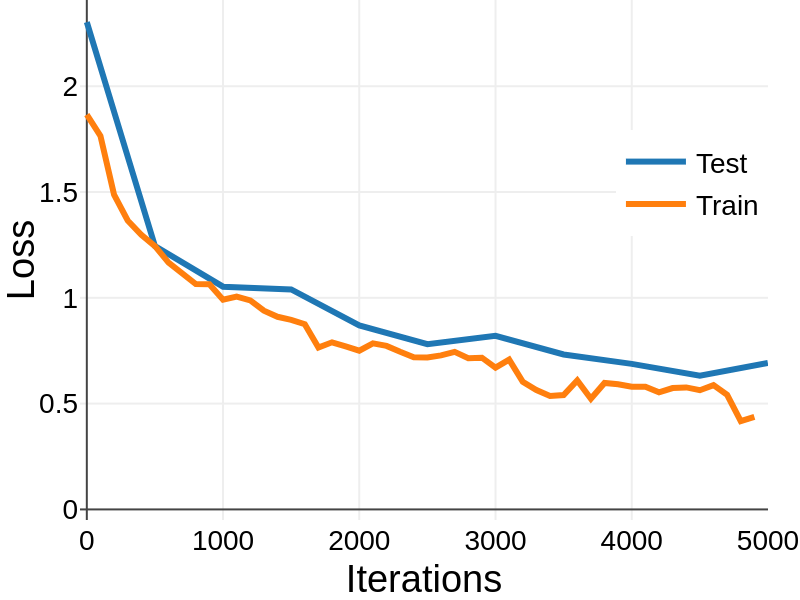
\includegraphics[scale=0.22]{img/convnet-loss}
\caption{}
\end{subfigure}
\begin{subfigure}{0.49\textwidth}
\centering
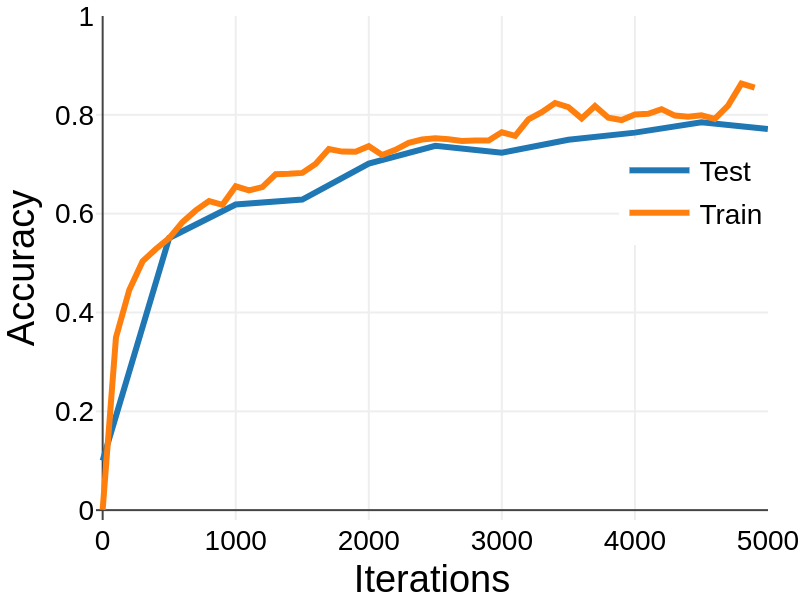
\includegraphics[scale=0.22]{img/convnet-acc}
\caption{}
\end{subfigure}
 \caption{Curves for (a) the loss, and (b) accuracy on the training and test splits for the CNN. Training values are averaged over 10 steps, and test values are measured every 100 steps.}
\label{fig:convnet_curves}
\end{figure}

\bibliographystyle{unsrt}
\bibliography{refs}


\end{document}
